\chapter{DNA प्रतिकृतिकरण और समसूत्री विभाजन}\label{ch:b1:replication-mitosis}

हर आठ घंटे के आसपास आँत के अस्तर की कोई \omterm{def:b1:cell-unit-of-life:cell}{कोशिका} छह अरब \omterm{thm:b1:nucleic-acids:helix}{क्षारक युग्मों} की
नक़ल करती है, और उसमें अरब में लगभग एक भूल होती है, फिर दोनों प्रतियाँ दो
संततियों में इस तरह छाँटती है कि हर एक को ठीक छियालीस \omterm{def:b1:genomes:genome}{गुणसूत्र} मिलें ---
न पैंतालीस, न सैंतालीस। नक़ल वह मशीन करती है जो एक लड़ी पढ़ती है और उसका
पूरक प्रति सेकंड पचास अक्षरों की दर से, एक साथ दसियों हज़ार आरंभ-बिंदुओं
से बनाती है; और छँटाई \omterm{def:b1:eukaryotic-cell:cytoskeleton}{सूक्ष्म नलिकाओं} का वह \omterm{def:b1:replication-mitosis:mitosis}{तर्कु} करता है जो हर \omterm{def:b1:genomes:genome}{गुणसूत्र}
की दोनों प्रतियाँ एक लाख विभाजनों में एक भूल की परिशुद्धता से अलग खींच
लेता है। यह अध्याय \omterm{def:b1:replication-mitosis:fork}{प्रतिकृतिकरण द्विशाख} और उसके \omterm{def:b1:enzymes:enzyme}{एंजाइमों}, सिरों की
समस्या, उस \omterm{def:b1:replication-mitosis:cycle}{कोशिका चक्र} का जो प्रतिकृतिकरण तथा विभाजन का समय तय करता है,
और स्वयं विभाजन यानी \omterm{def:b1:replication-mitosis:mitosis}{समसूत्री विभाजन} का वर्णन करता है।

\section{अर्ध-संरक्षी प्रतिकृतिकरण}

\begin{proposition}[हर लड़ी एक साँचा है]\label{prop:b1:replication-mitosis:semiconservative}
\index{अर्ध-संरक्षी प्रतिकृतिकरण}
\omterm{def:b1:nucleic-acids:chain}{DNA} \emph{अर्ध-संरक्षी} रूप से प्रतिकृत होता है: कुंडली की दोनों लड़ियाँ
अलग होती हैं, और हर एक उस साँचे का काम करती है जिस पर एक नई पूरक लड़ी
बनाई जाती है, इसलिए हर संतति अणु एक पुरानी लड़ी और एक नई लड़ी का युग्म
होता है।
\end{proposition}
\begin{proof}[साक्ष्य]
मेसेल्सन और स्टाल (1958; जो लाइसेयी खंड से याद है) ने
\emph{E. coli} को भारी नाइट्रोजन पर उगाया, फिर हल्की नाइट्रोजन पर
पहुँचाया, और \omterm{def:b1:nucleic-acids:chain}{DNA} को घनत्व से अलग किया: एक पीढ़ी बाद सारा \omterm{def:b1:nucleic-acids:chain}{DNA}
मध्यवर्ती घनत्व का था, और दो पीढ़ी बाद आधा मध्यवर्ती तथा आधा हल्का ---
यानी ठीक वही भविष्यवाणी जो प्रति अणु एक पुरानी और एक नई लड़ी की है, और
किसी और योजना की नहीं। केर्न्स (1963) ने प्रतिकृत होते जीवाणु \omterm{def:b1:genomes:genome}{गुणसूत्रों}
को ट्रिटियम से चिह्नित किया और उन्हें स्वप्रकाशचित्रिकी से चित्रित किया:
ऐसे वृत्त जिनमें प्रतिकृत होता एक ``बुलबुला'' था और जिसके दोनों द्विशाख
एक उद्गम से विपरीत दिशाओं में चल रहे थे। कोर्नबर्ग (1956) ने ऐसा \omterm{def:b1:enzymes:enzyme}{एंजाइम}
शुद्ध किया जो परखनली में चारों न्यूक्लियोसाइड ट्राइफ़ॉस्फ़ेटों और किसी
साँचे से \omterm{def:b1:nucleic-acids:chain}{DNA} संश्लेषित करता था, साँचे के ही अनुक्रम में।
\end{proof}

\begin{definition}[प्रतिकृतिकरण द्विशाख और उसके एंजाइम]\label{def:b1:replication-mitosis:fork}
\index{प्रतिकृतिकरण द्विशाख}\index{DNA पॉलिमरेज़}\index{ओकाज़ाकी खंड}
प्रतिकृतिकरण किसी \emph{उद्गम} से शुरू होता है --- जीवाणु \omterm{def:b1:genomes:genome}{गुणसूत्र} पर
एक, किसी \omterm{def:b1:cell-unit-of-life:prokeuk}{सुकेंद्रकी} \omterm{def:b1:genomes:genome}{जीनोम} पर दसियों हज़ार --- जहाँ कुंडली खोली जाती है
और दो \emph{प्रतिकृतिकरण द्विशाख} विपरीत दिशाओं में चल पड़ते हैं। हर
द्विशाख पर: कोई \emph{हेलिकेज़} कुंडली खोलता है (प्रति \omterm{thm:b1:nucleic-acids:helix}{क्षारक युग्म} एक
\omterm{def:b1:water-small-molecules:atp}{ATP}), \emph{एकलड़ी बंधनकारी \omterm{def:b1:proteins:peptide}{प्रोटीन}} अलग हुई लड़ियों को अलग रखते हैं, और
द्विशाख से आगे कोई \emph{टोपोआइसोमरेज़} उस ऐंठन को ढीला करता है जो खुलने
से जमा होती जाती है। \emph{\omterm{def:b1:nucleic-acids:chain}{DNA} पॉलिमरेज़} \omterm{def:b1:nucleic-acids:nucleotide}{न्यूक्लियोटाइड} केवल किसी
मौजूदा शृंखला के $3'$ हाइड्रॉक्सिल पर जोड़ता है, इसलिए हर नई लड़ी
$5' \to 3'$ बढ़ती है और कोई भी शून्य से शुरू नहीं हो सकती: पहले कोई
\emph{प्राइमेज़} एक छोटा \omterm{def:b1:nucleic-acids:chain}{RNA} \emph{प्राइमर} बिछाता है जिसे पॉलिमरेज़
बढ़ाता है। जिस साँचे को $3' \to 5'$ पढ़ा जाता है उस पर नई लड़ी द्विशाख
की ओर सतत बढ़ती है: यही \emph{अग्रणी लड़ी} है।
दूसरे साँचे पर नई लड़ी को द्विशाख से दूर की ओर बढ़ना पड़ता है, और वह
जीवाणुओं में \qtyrange{1000}{2000}{} तथा \omterm{def:b1:cell-unit-of-life:prokeuk}{सुकेंद्रकियों} में
\qtyrange{100}{200}{} \omterm{def:b1:nucleic-acids:nucleotide}{न्यूक्लियोटाइडों} के टुकड़ों में बढ़ती है, यानी
\emph{ओकाज़ाकी खंडों} में, और हर खंड का अपना प्राइमर होता है: यही
\emph{पश्चगामी लड़ी} है। कोई दूसरा पॉलिमरेज़ प्राइमरों की जगह \omterm{def:b1:nucleic-acids:chain}{DNA} रख देता
है और कोई \emph{लाइगेज़} उन खंडों को एक लड़ी में सील कर देता है।
\end{definition}

\begin{omfigure}
\begin{tikzpicture}[font=\footnotesize, >=Stealth, line cap=round]
  % parental duplex on the right, opening leftward
  \draw[very thick, omDef] (12.4,1.0) -- (7.6,1.0);
  \draw[very thick, omDef!50] (12.4,-1.0) -- (7.6,-1.0);
  \foreach \x in {8.0,8.6,...,12.2} { \draw[thick, gray!60] (\x,1.0) -- (\x,-1.0); }
  \node[anchor=south] at (10.0,1.15) {जनक द्विलड़ी};
  % helicase at the fork
  \node[circle, draw, thick, fill=omProp!40, minimum size=9mm, font=\scriptsize] (hel) at (7.3,0) {हेलिकेज़};
  \draw[->, very thick, omProp!80!black] (6.4,-1.9) -- (5.2,-1.9) node[left, font=\scriptsize] {द्विशाख चलता है};
  % separated template strands going left
  \draw[very thick, omDef] (7.0,0.55) .. controls (5.5,1.5) .. (0.4,2.2);
  \draw[very thick, omDef!50] (7.0,-0.55) .. controls (5.5,-1.5) .. (0.4,-2.2);
  \node[anchor=east, omDef] at (0.3,2.2) {$3'$};
  \node[anchor=east, omDef!70!black] at (0.3,-2.2) {$5'$};
  % leading strand: continuous new strand along upper template
  \draw[very thick, omThm] (1.0,1.85) .. controls (4.5,1.35) .. (6.2,0.75);
  \node[draw, thick, fill=omThm!25, rounded corners=3pt, inner sep=2pt, font=\scriptsize] at (6.0,0.95) {पॉल};
  \node[anchor=south west, omThm, align=left] at (1.0,2.35) {अग्रणी लड़ी: सतत, द्विशाख की ओर $5' \to 3'$};
  \node[anchor=east, omThm] at (0.95,1.85) {$5'$};
  % lagging strand: Okazaki fragments along lower template, each with a primer
  \foreach \x/\y in {1.2/-1.95, 3.3/-1.55, 5.3/-1.05} {
    \fill[omExo!80!black] (\x,\y) circle (0.08);
    \draw[very thick, omThm] (\x,\y) .. controls (\x+0.8,\y+0.15) .. (\x+1.5,\y+0.25);
  }
  \node[draw, thick, fill=omThm!25, rounded corners=3pt, inner sep=2pt, font=\scriptsize] at (6.7,-1.0) {पॉल};
  \node[anchor=north west, align=left] at (1.0,-2.5) {पश्चगामी लड़ी: ओकाज़ाकी खंड, हर एक किसी RNA प्राइमर (\textcolor{omExo!80!black}{बिंदु}) से शुरू,\\ द्विशाख से दूर $5' \to 3'$ बढ़ते; प्राइमर बदले जाते हैं, खंड लाइगेज़ से जोड़े जाते हैं};
  \node[font=\scriptsize, anchor=south] at (3.3,-1.35) {$5'$};
\end{tikzpicture}

{\small एक \omterm{def:b1:replication-mitosis:fork}{प्रतिकृतिकरण द्विशाख}। हेलिकेज़ जनक द्विलड़ी खोलता है;
अग्रणी लड़ी द्विशाख की ओर सतत नक़ल होती है, और पश्चगामी लड़ी पीछे की ओर
\omterm{def:b1:replication-mitosis:fork}{ओकाज़ाकी खंडों} में, क्योंकि पॉलिमरेज़ केवल $5' \to 3'$ दिशा में ही
बनाते हैं।}
\end{omfigure}

\begin{proposition}[सत्यनिष्ठा]\label{prop:b1:replication-mitosis:fidelity}
\index{प्रूफ़-पठन}
अकेला क्षारक-युग्मन $10^5$ में लगभग एक भूल देता; पॉलिमरेज़
\emph{प्रूफ़-पठन} करता है --- कोई $3' \to 5'$ बहिर्न्यूक्लिएज़ क्रिया
अगला \omterm{def:b1:nucleic-acids:nucleotide}{न्यूक्लियोटाइड} जुड़ने से पहले बेमेल \omterm{def:b1:nucleic-acids:nucleotide}{न्यूक्लियोटाइड} हटा देती है ---
जिससे भूल $10^7$ में एक रह जाती है; और द्विशाख के गुज़र जाने के बाद कोई
\emph{बेमेल मरम्मत} तंत्र बचे हुए बेमेल ढूँढ़ता है, नई लड़ी पहचानता है,
और उसे सुधार देता है: यानी प्रति प्रतिकृतिकरण $10^9$ से $10^{10}$ \omterm{thm:b1:nucleic-acids:helix}{क्षारक
युग्मों} में एक भूल। $\num{6.4e9}$ युग्म नक़ल करती कोई मानव \omterm{def:b1:cell-unit-of-life:cell}{कोशिका} हर बार
विभाजित होने पर मुट्ठी भर उत्परिवर्तन करती है; और कोई जीवाणु, एक हज़ार
विभाजनों में एक।
\end{proposition}

\begin{example}[चाल और आरंभ-बिंदु]\label{ex:b1:replication-mitosis:speed}
कोई जीवाणु द्विशाख प्रति सेकंड \qty{1000}{} \omterm{thm:b1:nucleic-acids:helix}{क्षारक युग्म} चलता है: दो
द्विशाख \emph{E. coli} की \qty{4.6}{Mb} \qty{40}{min} में नक़ल कर लेते
हैं, और समृद्ध माध्यम में, जहाँ \omterm{def:b1:cell-unit-of-life:cell}{कोशिका} हर बीस मिनट में विभाजित होती है,
नया चक्कर पिछले के समाप्त होने से पहले ही शुरू हो जाता है। कोई \omterm{def:b1:cell-unit-of-life:prokeuk}{सुकेंद्रकी}
द्विशाख, जिसे क्रोमैटिन धीमा कर देती है, प्रति सेकंड \qty{50}{} चलता है:
\qty{250}{Mb} के किसी मानव \omterm{def:b1:genomes:genome}{गुणसूत्र} को एक उद्गम से नक़ल करने में महीना लग
जाता, इसलिए \omterm{def:b1:genomes:genome}{जीनोम} कोई \num{40000} उद्गमों से आठ घंटे में नक़ल किया जाता
है, और वह भी हर कोशिका-प्रकार के लिए नियत क्रम में।
\end{example}

\section{सिरे}

\begin{proposition}[सिरा-प्रतिकृतिकरण की समस्या और टीलोमरेज़]\label{prop:b1:replication-mitosis:telomerase}
\index{टीलोमरेज़}
किसी रैखिक \omterm{def:b1:genomes:genome}{गुणसूत्र} पर पश्चगामी लड़ी बिलकुल सिरे तक पूरी नहीं की जा
सकती: जब अंतिम प्राइमर हटाया जाता है तब ऊपर की ओर कोई ऐसा $3'$
हाइड्रॉक्सिल नहीं होता जिससे वह ख़ाली जगह भरी जा सके, और हर
प्रतिकृतिकरण \omterm{def:b1:genomes:genome}{गुणसूत्र} को \qtyrange{50}{100}{} \omterm{def:b1:nucleic-acids:nucleotide}{न्यूक्लियोटाइड} छोटा कर
देता। \omterm{def:b1:cell-unit-of-life:prokeuk}{सुकेंद्रकी} अपने \omterm{def:b1:genomes:genome}{गुणसूत्रों} के सिरों पर \emph{\omterm{def:b1:genomes:karyotype}{टीलोमियर}} रखते हैं,
यानी किसी छोटी पुनरावृत्ति (कशेरुकियों में TTAGGG) की हज़ारों प्रतियाँ,
जिन पर कोई \omterm{def:b1:genomes:gene}{जीन} नहीं होते, और जनन \omterm{def:b1:cell-unit-of-life:cell}{कोशिकाएँ} तथा मूल \omterm{def:b1:cell-unit-of-life:cell}{कोशिकाएँ}
\emph{टीलोमरेज़} ढोती हैं, यानी वह \omterm{def:b1:enzymes:enzyme}{एंजाइम} जिसका अपना \omterm{def:b1:nucleic-acids:chain}{RNA} साँचा है और जो
$3'$ सिरे पर पुनरावृत्तियाँ जोड़ देता है और वह लौटा देता है जो
प्रतिकृतिकरण खोता है। अधिकांश कायिक \omterm{def:b1:cell-unit-of-life:cell}{कोशिकाओं} में वह नहीं होता: उनके
\omterm{def:b1:genomes:karyotype}{टीलोमियर} हर विभाजन पर छोटे होते जाते हैं, और संवर्धन में कोई पचास विभाजनों
के बाद वे विभाजित होना बंद कर देती हैं। जीवाणुओं के, जिनके \omterm{def:b1:genomes:genome}{गुणसूत्र} वर्तुल
हैं, कोई सिरे ही नहीं होते।
\end{proposition}

\begin{omfigure}
\begin{tikzpicture}[font=\footnotesize, >=Stealth, line cap=round]
  % top: the problem
  \draw[very thick, omDef] (0,1.2) -- (8,1.2) node[right] {$3'$ (साँचा)};
  \draw[very thick, omThm] (0,0.8) -- (6.3,0.8);
  \fill[omExo!80!black] (6.3,0.8) circle (0.08); \draw[very thick, omExo!80!black] (6.3,0.8) -- (7.0,0.8);
  \node[anchor=east, omThm] at (-0.1,0.8) {नई पश्चगामी लड़ी $5'$};
  \node[anchor=north, font=\scriptsize, omExo!80!black] at (6.65,0.72) {अंतिम प्राइमर};
  \draw[thick, gray] (7.0,0.55) -- (8.0,0.55);
  \node[anchor=north, font=\scriptsize, align=center, gray] at (7.5,0.45) {ख़ाली जगह: प्राइमर हटते ही\\ बढ़ाने को कुछ नहीं बचता};
  % bottom: telomerase
  \draw[very thick, omDef] (0,-1.6) -- (8,-1.6);
  \draw[very thick, omDef, dashed] (8,-1.6) -- (10.2,-1.6) node[right] {$3'$ बढ़ाया गया};
  \node[draw, thick, fill=omProp!30, rounded corners=4pt, inner sep=3pt, align=center, font=\scriptsize] at (9.1,-0.95) {टीलोमरेज़\\ (भीतर RNA साँचा)};
  \draw[very thick, omThm] (0,-2.0) -- (6.3,-2.0);
  \draw[very thick, omThm, dashed] (6.3,-2.0) -- (8.6,-2.0);
  \node[anchor=east, align=right, font=\scriptsize] at (-0.1,-1.8) {टीलोमियर पुनरावृत्तियाँ\\ TTAGGG\ldots};
  \node[anchor=north, align=center, gray] at (5,-2.3) {टीलोमरेज़ साँचे का $3'$ सिरा पुनरावृत्तियों से लंबा करता है; उस बढ़ाव पर एक नया\\ प्राइमर पश्चगामी लड़ी को मूल लंबाई तक पूरा होने देता है};
\end{tikzpicture}

{\small सिरा-प्रतिकृतिकरण की समस्या (ऊपर) और उसका समाधान (नीचे)।
पश्चगामी लड़ी \omterm{def:b1:genomes:genome}{गुणसूत्र} के सिरे पर छोटी रह जाती है; और टीलोमरेज़ साँचे के
$3'$ सिरे पर पुनरावृत्तियाँ जोड़ देता है ताकि हानि उस अनुक्रम पर पड़े जिस
पर कोई \omterm{def:b1:genomes:gene}{जीन} नहीं है।}
\end{omfigure}

\section{कोशिका चक्र}

\begin{definition}[कोशिका चक्र]\label{def:b1:replication-mitosis:cycle}
\index{कोशिका चक्र}\index{अंतरावस्था}
किसी \omterm{def:b1:cell-unit-of-life:prokeuk}{सुकेंद्रकी कोशिका} के \emph{\omterm{def:b1:cell-unit-of-life:cell}{कोशिका} चक्र} की चार प्रावस्थाएँ हैं।
\emph{G$_1$} (अंतराल 1): \omterm{def:b1:cell-unit-of-life:cell}{कोशिका} बढ़ती है और प्रतिकृतिकरण के \omterm{def:b1:enzymes:enzyme}{एंजाइम} बनाती
है; \emph{S} (संश्लेषण): वह अपना \omterm{def:b1:nucleic-acids:chain}{DNA} प्रतिकृत करती है, जिससे हर
\omterm{def:b1:genomes:genome}{गुणसूत्र} \omterm{def:b1:genomes:karyotype}{सेंट्रोमियर} पर जुड़ी दो एक जैसी \emph{सहोदर \omterm{def:b1:replication-mitosis:mitosis}{क्रोमैटिडें}} बन जाता
है; \emph{G$_2$}: वह और बढ़ती है और प्रतियाँ जाँचती है;
\emph{M}: \emph{\omterm{def:b1:replication-mitosis:mitosis}{समसूत्री विभाजन}}, यानी केंद्रक का विभाजन, और उसके बाद
\emph{कोशिकाद्रव्य-विभाजन}, यानी \omterm{def:b1:cell-unit-of-life:cell}{कोशिकाद्रव्य} का विभाजन। G$_1$, S और
G$_2$ मिलकर \emph{अंतरावस्था} हैं, जिसमें \omterm{def:b1:genomes:genome}{गुणसूत्र} फैले और सक्रिय रहते
हैं; और जो \omterm{def:b1:cell-unit-of-life:cell}{कोशिका} विभाजित होना बंद कर देती है वह G$_1$ से निकलकर किसी
विश्राम अवस्था, G$_0$, में चली जाती है। विभाजित होती किसी मानव \omterm{def:b1:cell-unit-of-life:cell}{कोशिका} को
लगभग \qty{24}{h} लगते हैं: G$_1$ \qty{10}{h}, S \qty{8}{h}, G$_2$ \qty{4}{h}, M
\qty{1}{h}; किसी खमीर को \qty{90}{min}; और किसी आरंभिक मेंढक-भ्रूण को तीस
मिनट, बिना किसी अंतराल के।
\end{definition}

\begin{omfigure}
\begin{tikzpicture}
\begin{axis}[
  width=0.9\linewidth, height=5.6cm,
  axis x line=bottom, axis y line=left,
  xmin=0, xmax=26, ymin=0, ymax=2.6,
  xlabel={समय (h)}, ylabel={प्रति केंद्रक DNA},
  xlabel style={font=\small, at={(axis description cs:0.5,-0.14)}, anchor=north},
  ylabel style={font=\small},
  tick label style={font=\small}, xtick={0,10,18,22,23,24}, xticklabels={0,10,18,22,23,24},
  ytick={1,2}, yticklabels={$q$,$2q$},
  clip=false,
]
\addplot[very thick, omDef] coordinates {(0,1) (10,1) (18,2) (23,2) (23.6,2) (23.6,1) (24,1) (26,1)};
\fill[omDef!12] (axis cs:0,2.25) rectangle (axis cs:10,2.55); \node[font=\scriptsize] at (axis cs:5,2.4) {G$_1$: वृद्धि};
\fill[omThm!15] (axis cs:10,2.25) rectangle (axis cs:18,2.55); \node[font=\scriptsize] at (axis cs:14,2.4) {S: प्रतिकृतिकरण};
\fill[omDef!12] (axis cs:18,2.25) rectangle (axis cs:22,2.55); \node[font=\scriptsize] at (axis cs:20,2.4) {G$_2$};
\fill[omExo!25] (axis cs:22,2.25) rectangle (axis cs:24,2.55); \node[font=\scriptsize] at (axis cs:23,2.4) {M};
\node[font=\scriptsize, anchor=west, align=left] at (axis cs:24.1,1.5) {दो कोशिकाएँ,\\ हर एक $q$};
\end{axis}
\end{tikzpicture}

{\small \qty{24}{h} के एक \omterm{def:b1:replication-mitosis:cycle}{कोशिका चक्र} में किसी केंद्रक की \omterm{def:b1:nucleic-acids:chain}{DNA} मात्रा।
वह S प्रावस्था के दौरान $q$ (एक \omterm{def:b1:replication-mitosis:mitosis}{क्रोमैटिड} के 2n \omterm{def:b1:genomes:genome}{गुणसूत्र}) से
$2q$ (दो \omterm{def:b1:replication-mitosis:mitosis}{क्रोमैटिडों} के 2n \omterm{def:b1:genomes:genome}{गुणसूत्र}) तक दुगुनी हो जाती है, और \omterm{def:b1:replication-mitosis:mitosis}{समसूत्री
विभाजन} के अंत में हर संतति में $q$ पर लौट आती है; और \omterm{def:b1:genomes:genome}{गुणसूत्रों} की संख्या
कभी नहीं बदलती।}
\end{omfigure}

\begin{proposition}[जाँच-बिंदु]\label{prop:b1:replication-mitosis:checkpoints}
\index{जाँच-बिंदु}
चक्र को \omterm{def:b1:proteins:peptide}{प्रोटीन} काइनेज़ों का एक कुल आगे धकेलता है, जिन्हें बारी-बारी से
\emph{साइक्लिन} कहलाते \omterm{def:b1:proteins:peptide}{प्रोटीन} सक्रिय करते हैं और जिनके स्तर चक्र भर
चढ़ते-उतरते रहते हैं, और वह \emph{जाँच-बिंदुओं} पर तब तक रोका जाता है जब
तक शर्तें पूरी न हों: G$_1$ के अंत में \omterm{def:b1:cell-unit-of-life:cell}{कोशिका} प्रतिकृतिकरण के लिए तभी
प्रतिबद्ध होती है जब वह पर्याप्त बड़ी हो, पोषित हो और विभाजित होने का
संकेत पा चुकी हो, और उसका \omterm{def:b1:nucleic-acids:chain}{DNA} अक्षत हो; G$_2$ के अंत में वह \omterm{def:b1:replication-mitosis:mitosis}{समसूत्री
विभाजन} में तभी घुसती है जब प्रतिकृतिकरण पूरा हो; और विभाजन में \omterm{def:b1:replication-mitosis:mitosis}{क्रोमैटिडें}
तभी अलग होती हैं जब हर \omterm{def:b1:genomes:genome}{गुणसूत्र} दोनों ओर से \omterm{def:b1:replication-mitosis:mitosis}{तर्कु} से जुड़ा हो। क्षति चक्र
रोक देती है और, यदि उसकी मरम्मत न हो सके, तो \omterm{def:b1:cell-unit-of-life:cell}{कोशिका} की मृत्यु करा देती
है। इस नियंत्रण की आणविक मशीनरी वर्ष 3 के खंड की है; और उसका चूकना कैंसर
है।
\end{proposition}

\section{समसूत्री विभाजन}

\begin{definition}[समसूत्री विभाजन]\label{def:b1:replication-mitosis:mitosis}
\index{समसूत्री विभाजन}\index{तर्कु}\index{क्रोमैटिड}
\emph{समसूत्री विभाजन} प्रतिकृत \omterm{def:b1:genomes:genome}{गुणसूत्रों} को इस तरह बाँटता है कि हर
संतति केंद्रक को हर \omterm{def:b1:genomes:genome}{गुणसूत्र} की एक क्रोमैटिड मिले --- यानी जनक जितनी ही
संख्या और वही \omterm{def:b1:genomes:gene}{जीन}। उसकी अवस्थाएँ:
\begin{itemize}
  \item \emph{पूर्वावस्था}: \omterm{def:b1:genomes:genome}{गुणसूत्र} संघनित होकर दिखने वाली छड़ें बन
        जाते हैं, और हर छड़ दो सहोदर क्रोमैटिडों की है जिन्हें कोहेसिन
        \omterm{def:b1:proteins:peptide}{प्रोटीन} उनकी पूरी लंबाई भर जोड़े रखते हैं; दोनों
        \emph{\omterm{def:b1:eukaryotic-cell:cytoskeleton}{तारककाय}} दूर हटते हैं और उनके बीच \omterm{def:b1:eukaryotic-cell:cytoskeleton}{सूक्ष्म नलिकाओं} का
        \emph{समसूत्री तर्कु} उगता है;
  \item \emph{पूर्वमध्यावस्था}: \omterm{def:b1:eukaryotic-cell:nucleus}{केंद्रक आवरण} टूट जाता है; और तर्कु की
        \omterm{def:b1:eukaryotic-cell:cytoskeleton}{सूक्ष्म नलिकाएँ} विपरीत ध्रुवों से हर क्रोमैटिड के
        \emph{गतिबिंदु} से जुड़ जाती हैं, जो \omterm{def:b1:genomes:karyotype}{सेंट्रोमियर} पर की एक
        \omterm{def:b1:proteins:peptide}{प्रोटीन} संरचना है;
  \item \emph{मध्यावस्था}: \omterm{def:b1:genomes:genome}{गुणसूत्र} तर्कु की भूमध्य रेखा पर पंक्तिबद्ध
        हो जाते हैं, और हर एक दोनों ध्रुवों से तनाव में रहता है;
  \item \emph{पश्चावस्था}: कोहेसिन काट दिया जाता है, सहोदर क्रोमैटिडें
        अलग होती हैं और \omterm{def:b1:eukaryotic-cell:cytoskeleton}{सूक्ष्म नलिकाओं} के छोटा होते जाने पर विपरीत
        ध्रुवों की ओर खींची जाती हैं (पश्चावस्था A) तथा ध्रुव दूर हटते
        हैं (पश्चावस्था B);
  \item \emph{अंत्यावस्था}: \omterm{def:b1:genomes:genome}{गुणसूत्र} फिर फैल जाते हैं, और हर समुच्चय के
        चारों ओर एक \omterm{def:b1:eukaryotic-cell:nucleus}{केंद्रक आवरण} फिर बन जाता है।
\end{itemize}
फिर \emph{कोशिकाद्रव्य-विभाजन} \omterm{def:b1:cell-unit-of-life:cell}{कोशिकाद्रव्य} को बाँटता है: जंतु \omterm{def:b1:cell-unit-of-life:cell}{कोशिकाओं}
में ऐक्टिन तथा मायोसिन की कोई \emph{संकुचनशील वलय} \omterm{def:b1:cell-unit-of-life:cell}{कोशिका} को चुटककर दो
कर देती है; और पादप \omterm{def:b1:cell-unit-of-life:cell}{कोशिकाओं} में \omterm{def:b1:eukaryotic-cell:endomembrane}{गॉल्जी} से आई पुटिकाएँ भूमध्य रेखा पर
जुड़कर एक \emph{\omterm{def:b1:cell-unit-of-life:cell}{कोशिका} पट्ट} बनाती हैं जो बाहर की ओर बढ़कर नई भित्ति बन
जाता है।
\end{definition}

\begin{omfigure}
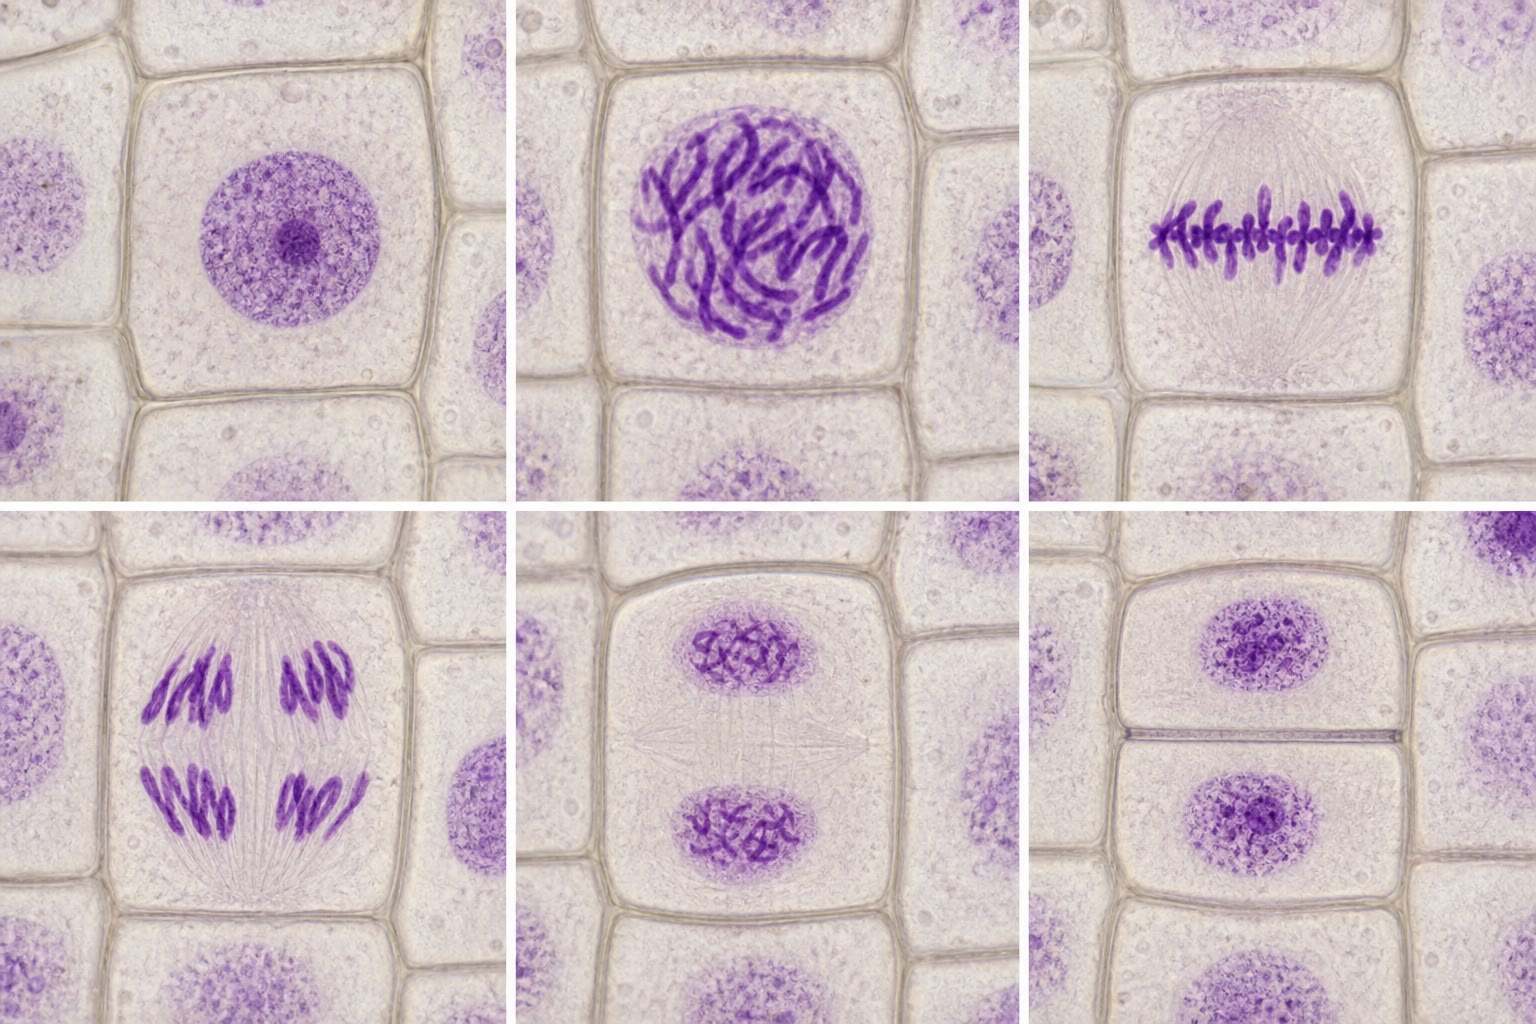
\includegraphics[width=0.9\linewidth]{images/book3/ai/b3-18-mitosis-grid.jpg}

{\small प्याज़ की जड़-सिरे की \omterm{def:b1:cell-unit-of-life:cell}{कोशिकाएँ} \omterm{def:b1:replication-mitosis:cycle}{अंतरावस्था}, पूर्वावस्था,
मध्यावस्था, पश्चावस्था, अंत्यावस्था में, और कोशिकाद्रव्य-विभाजन के बाद
बीच में नई भित्ति के साथ। \omterm{def:b1:genomes:genome}{गुणसूत्र} केवल तभी दिखते हैं जब वे संघनित हों,
यानी पूर्वावस्था से अंत्यावस्था तक।}
\end{omfigure}

\begin{omfigure}
\begin{tikzpicture}[font=\footnotesize, >=Stealth, line cap=round]
  \foreach \i/\name in {0/पूर्वावस्था, 1/मध्यावस्था, 2/पश्चावस्था, 3/अंत्यावस्था} {
    \begin{scope}[xshift=\i*3.3cm]
      \draw[thick, omDef!70!black, fill=omDef!5] (0,0) ellipse (1.4 and 1.1);
      \node[anchor=north] at (0,-1.2) {\name};
    \end{scope}
  }
  % prophase: two centrosomes, condensed chromosomes (X shapes) scattered, envelope
  \begin{scope}
    \draw[thick, gray, dashed] (0,0) circle (0.8);
    \foreach \p/\a in {(-0.3,0.25)/30, (0.35,-0.1)/-40, (0.05,-0.45)/80} { \draw[very thick, omThm] \p ++(\a:0.22) -- ++(\a+180:0.44); \draw[very thick, omThm] \p ++(\a+60:0.22) -- ++(\a+240:0.44); }
    \fill[omProp!80!black] (-1.1,0.6) circle (0.07); \fill[omProp!80!black] (1.1,-0.6) circle (0.07);
    \foreach \a in {-30,0,30} { \draw[omProp!60!black] (-1.1,0.6) -- ++(\a-20:0.45); \draw[omProp!60!black] (1.1,-0.6) -- ++(\a+160:0.45); }
  \end{scope}
  % metaphase: spindle pole to pole, chromosomes on the plate
  \begin{scope}[xshift=3.3cm]
    \fill[omProp!80!black] (-1.25,0) circle (0.07); \fill[omProp!80!black] (1.25,0) circle (0.07);
    \foreach \y in {-0.5,-0.25,0,0.25,0.5} { \draw[omProp!60!black] (-1.25,0) -- (0,\y); \draw[omProp!60!black] (1.25,0) -- (0,\y); }
    \foreach \y in {-0.5,-0.17,0.17,0.5} { \draw[very thick, omThm] (-0.12,\y-0.14) -- (0.12,\y+0.14); \draw[very thick, omThm] (-0.12,\y+0.14) -- (0.12,\y-0.14); }
  \end{scope}
  % anaphase: chromatids moving to poles (V shapes)
  \begin{scope}[xshift=6.6cm]
    \fill[omProp!80!black] (-1.25,0) circle (0.07); \fill[omProp!80!black] (1.25,0) circle (0.07);
    \foreach \y in {-0.45,-0.15,0.15,0.45} { \draw[omProp!60!black] (-1.25,0) -- (-0.55,\y); \draw[omProp!60!black] (1.25,0) -- (0.55,\y); \draw[very thick, omThm] (-0.55,\y) -- (-0.35,\y+0.12) (-0.55,\y) -- (-0.35,\y-0.12); \draw[very thick, omThm] (0.55,\y) -- (0.35,\y+0.12) (0.55,\y) -- (0.35,\y-0.12); }
  \end{scope}
  % telophase: two nuclei reforming, cleavage furrow
  \begin{scope}[xshift=9.9cm]
    \draw[thick, gray, dashed] (-0.7,0) circle (0.45); \draw[thick, gray, dashed] (0.7,0) circle (0.45);
    \foreach \x in {-0.8,-0.6,0.6,0.8} { \draw[thick, omThm] (\x,-0.2) -- (\x,0.2); }
    \draw[very thick, omExo!70!black] (0,1.1) -- (0,0.55); \draw[very thick, omExo!70!black] (0,-1.1) -- (0,-0.55);
    \node[font=\scriptsize, omExo!70!black, anchor=south] at (0,1.15) {खाँच};
  \end{scope}
\end{tikzpicture}

{\small किसी जंतु \omterm{def:b1:cell-unit-of-life:cell}{कोशिका} में \omterm{def:b1:replication-mitosis:mitosis}{समसूत्री विभाजन} की चार अवस्थाएँ।
पूर्वावस्था: दोनों तारककायों से \omterm{def:b1:replication-mitosis:mitosis}{तर्कु} बनते समय \omterm{def:b1:genomes:genome}{गुणसूत्र} संघनित होते हैं।
मध्यावस्था: हर \omterm{def:b1:genomes:genome}{गुणसूत्र} भूमध्य रेखा पर बैठा है, दोनों ध्रुवों से जुड़ा।
पश्चावस्था: सहोदर \omterm{def:b1:replication-mitosis:mitosis}{क्रोमैटिडें} अलग खींची जाती हैं। अंत्यावस्था:
दो केंद्रक फिर बनते हैं और खाँच \omterm{def:b1:cell-unit-of-life:cell}{कोशिका} को बाँट देती है।}
\end{omfigure}

\begin{omfigure}
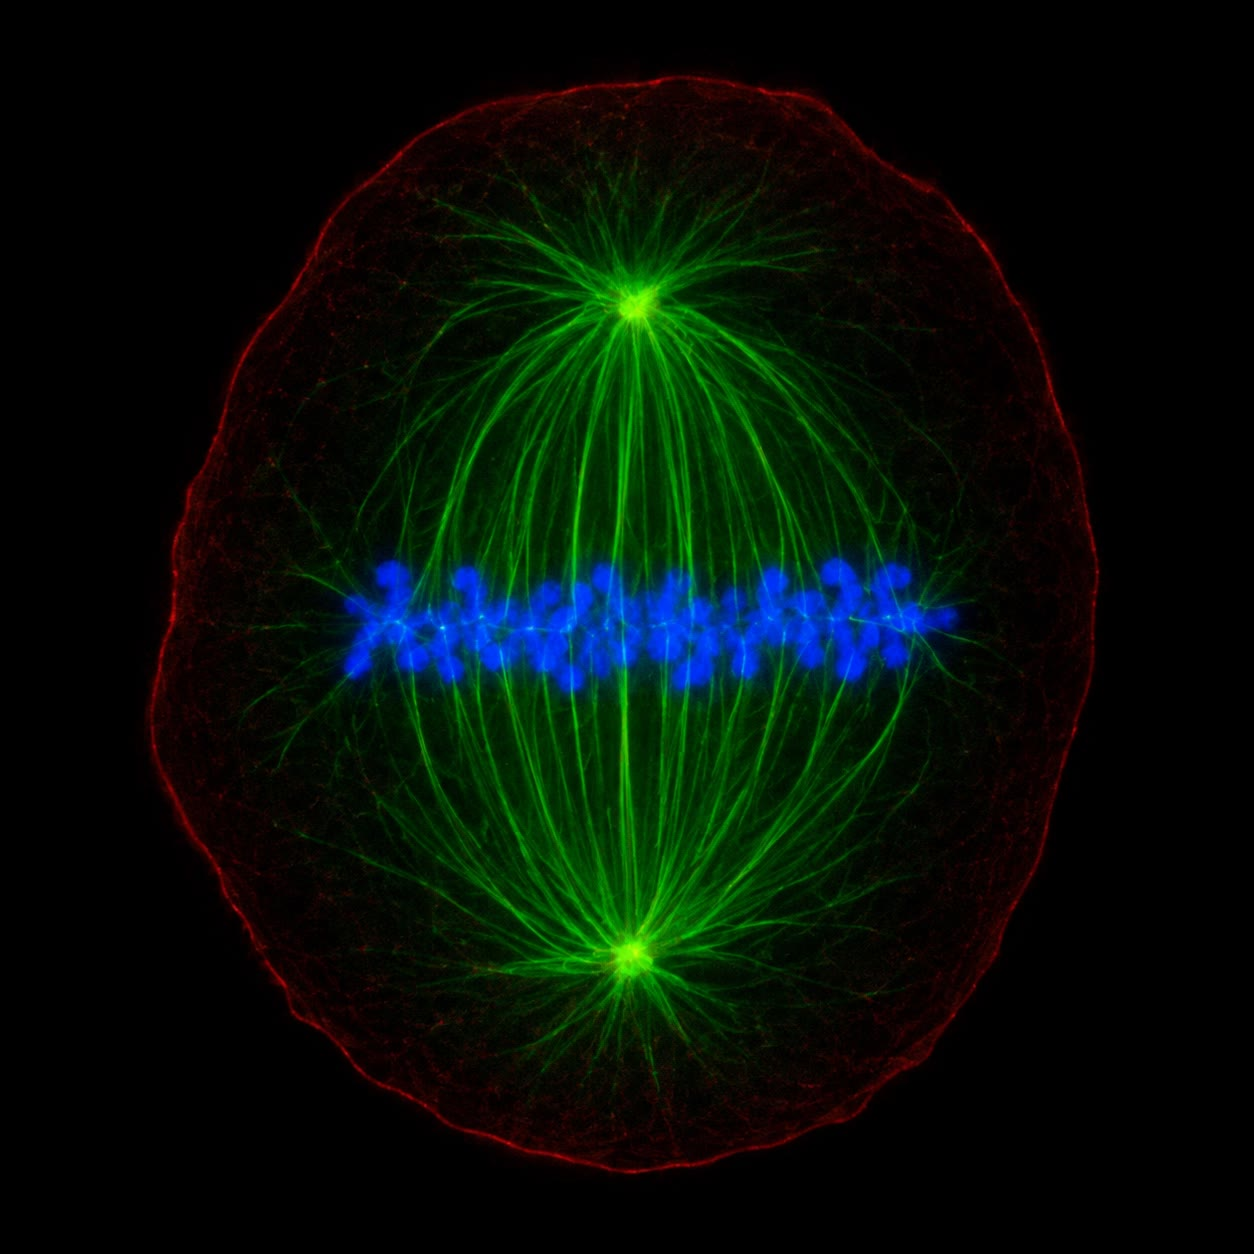
\includegraphics[width=0.4\linewidth]{images/book3/ai/b3-18-mitotic-spindle-fluorescence.jpg}

{\small मध्यावस्था पर संवर्धित एक \omterm{def:b1:cell-unit-of-life:cell}{कोशिका}, जिसकी \omterm{def:b1:eukaryotic-cell:cytoskeleton}{सूक्ष्म नलिकाएँ} हरी और
\omterm{def:b1:genomes:genome}{गुणसूत्र} नीले चिह्नित हैं: \omterm{def:b1:replication-mitosis:mitosis}{तर्कु} \omterm{def:b1:cell-unit-of-life:cell}{कोशिका} को ध्रुव से ध्रुव तक पार करता है
और \omterm{def:b1:genomes:genome}{गुणसूत्र} उसकी भूमध्य रेखा पर एक पट्ट बनाते हैं।}
\end{omfigure}

\begin{proposition}[समसूत्री विभाजन क्या संरक्षित करता है]\label{prop:b1:replication-mitosis:conserves}
\omterm{def:b1:replication-mitosis:mitosis}{समसूत्री विभाजन} वह विभाजन है जो \omterm{def:b1:genomes:genome}{गुणसूत्र} संख्या संरक्षित करता है: 2n
\omterm{def:b1:genomes:genome}{गुणसूत्रों} (मनुष्य में 46) वाली कोई \omterm{def:b1:cell-unit-of-life:cell}{कोशिका} 2n वाली दो \omterm{def:b1:cell-unit-of-life:cell}{कोशिकाएँ} देती है।
\omterm{def:b1:nucleic-acids:chain}{DNA} की मात्रा $2q$ (प्रतिकृतिकरण के बाद) से हर संतति में $q$ हो जाती है;
\omterm{def:b1:genomes:genome}{गुणसूत्रों} की संख्या कभी नहीं बदलती, क्योंकि \omterm{def:b1:genomes:genome}{गुणसूत्र} उसके \omterm{def:b1:genomes:karyotype}{सेंट्रोमियर} से
गिना जाता है, और हर \omterm{def:b1:replication-mitosis:mitosis}{क्रोमैटिड}, अलग होते ही, एक \omterm{def:b1:genomes:genome}{गुणसूत्र} है। इस तरह किसी
शरीर की हर \omterm{def:b1:cell-unit-of-life:cell}{कोशिका} उस अंडे के आनुवंशिक रूप से समान है जिससे वह उतरी है,
सिवाय उन उत्परिवर्तनों के जो नक़ल ने डाले हैं। जो विभाजन \omterm{def:b1:genomes:genome}{गुणसूत्र} संख्या
आधी करता है, यानी अर्धसूत्री विभाजन, वह वर्ष 2 के खंड का है।
\end{proposition}

\begin{method}[किसी कोशिका-चक्र प्रयोग को पढ़ना]\label{met:b1:replication-mitosis:reading}
\begin{enumerate}
  \item प्रति \omterm{def:b1:cell-unit-of-life:cell}{कोशिका} \omterm{def:b1:nucleic-acids:chain}{DNA} मापिए (कोई ऐसा रंजक जिसकी प्रतिदीप्ति \omterm{def:b1:nucleic-acids:chain}{DNA} के
        समानुपाती हो, कोशिका-दर-कोशिका): $q$ पर की \omterm{def:b1:cell-unit-of-life:cell}{कोशिकाएँ} G$_1$ में
        हैं, $2q$ पर G$_2$ या M में, और बीच वाली S में। भिन्न अवधियाँ
        दे देते हैं: किसी प्रावस्था का चक्र में हिस्सा उसका \omterm{def:b1:cell-unit-of-life:cell}{कोशिकाओं} में
        हिस्सा ही है।
  \item चिह्नित \omterm{def:b1:nucleic-acids:nucleotide}{न्यूक्लियोटाइड} (ब्रोमोडिऑक्सीयूरिडीन) का एक स्पंद दीजिए:
        उसे केवल S प्रावस्था की \omterm{def:b1:cell-unit-of-life:cell}{कोशिकाएँ} लेती हैं; चिह्नित भिन्न ही
        S भिन्न है, और चिह्न का \omterm{def:b1:replication-mitosis:mitosis}{समसूत्री विभाजन} तक पीछा करने से G$_2$ की
        लंबाई मिल जाती है।
  \item किसी रंगे हुए काट में समसूत्री आकृतियाँ गिनिए: \emph{समसूत्री
        सूचकांक}, यानी M में \omterm{def:b1:cell-unit-of-life:cell}{कोशिकाओं} का भिन्न, चक्र का वह भिन्न है जो M
        घेरता है --- एक घंटे के विभाजन वाले \qty{24}{h} के चक्र के लिए
        \qty{4}{\%}।
  \item किसी चरण को रोकिए (कोई दवा जो \omterm{def:b1:eukaryotic-cell:cytoskeleton}{सूक्ष्म नलिकाएँ} विबहुलकित करती है
        \omterm{def:b1:cell-unit-of-life:cell}{कोशिकाओं} को मध्यावस्था में रोक देती है; और जो \omterm{def:b1:nucleic-acids:chain}{DNA} संश्लेषण रोकती
        है उन्हें S में) और देखिए कि क्या जमा होता है।
\end{enumerate}
\end{method}

\begin{example}[आवर्तन]\label{ex:b1:replication-mitosis:turnover}
छोटी आँत की \omterm{def:b1:body-plans-tissues:epithelium}{उपकला} हर चार दिन में नई हो जाती है, त्वचा हर महीने, और लाल
\omterm{def:b1:cell-unit-of-life:cell}{कोशिकाएँ} हर चार महीने में मज्जा से, जो प्रति सेकंड बीस लाख बनाती है;
कोई यकृत \omterm{def:b1:cell-unit-of-life:cell}{कोशिका} साल में एक बार के आसपास विभाजित होती है और कोई \omterm{def:b1:body-plans-tissues:nervous}{न्यूरॉन}
कभी नहीं। किसी अर्बुद की \omterm{def:b1:cell-unit-of-life:cell}{कोशिकाएँ} अपने जाँच-बिंदु खो चुकी हैं: वे तब
विभाजित होती हैं जब उन्हें नहीं होना चाहिए, ग़लत छँटे \omterm{def:b1:genomes:genome}{गुणसूत्र} सह लेती
हैं, और वे उत्परिवर्तन जमा करती जाती हैं जो उन्हें और तेज़ विभाजित होने
देते हैं। कीमोथेरैपी इसी फ़र्क़ का लाभ उठाती है: जो दवाएँ \omterm{def:b1:replication-mitosis:mitosis}{तर्कु} या
पॉलिमरेज़ को विषाक्त करती हैं वे उन्हीं \omterm{def:b1:cell-unit-of-life:cell}{कोशिकाओं} को मारती हैं जो सबसे
अधिक विभाजित होती हैं।
\end{example}

\section{अभ्यास}

\begin{exercise}[$\star$]\label{exo:b1:replication-mitosis:1}
समझाइए कि किसी द्विशाख पर एक लड़ी सतत और दूसरी टुकड़ों में क्यों नक़ल
होती है।
\end{exercise}

\begin{exercise}[$\star$]\label{exo:b1:replication-mitosis:2}
किसी \omterm{def:b1:replication-mitosis:fork}{प्रतिकृतिकरण द्विशाख} के \omterm{def:b1:enzymes:enzyme}{एंजाइम} तथा \omterm{def:b1:proteins:peptide}{प्रोटीन} गिनाइए और हर एक का काम
बताइए।
\end{exercise}

\begin{exercise}[$\star$]\label{exo:b1:replication-mitosis:3}
DNA-मात्रा वाले आलेख से G$_1$, G$_2$ में और \omterm{def:b1:replication-mitosis:mitosis}{समसूत्री विभाजन} के बाद \omterm{def:b1:nucleic-acids:chain}{DNA}
की मात्रा पढ़िए, और हर एक में \omterm{def:b1:genomes:genome}{गुणसूत्रों} की संख्या भी।
\end{exercise}

\begin{exercise}[$\star$]\label{exo:b1:replication-mitosis:4}
\omterm{def:b1:replication-mitosis:mitosis}{समसूत्री विभाजन} की अवस्थाएँ क्रम में रखिए और हर एक की परिभाषक घटना दीजिए।
\end{exercise}

\begin{exercise}[$\star\star$]\label{exo:b1:replication-mitosis:5}
मानव \omterm{def:b1:genomes:genome}{जीनोम} की नक़ल में बने \omterm{def:b1:replication-mitosis:fork}{ओकाज़ाकी खंडों} की संख्या निकालिए
(\num{6.4e9} युग्म, \qty{150}{} के खंड), और इससे निकलती प्राइमरों,
प्राइमर-हटावों तथा जोड़ों की संख्या भी।
\end{exercise}

\begin{exercise}[$\star\star$]\label{exo:b1:replication-mitosis:6}
अकेले किसी पॉलिमरेज़ ($10^{-5}$) के लिए, प्रूफ़-पठन के साथ ($10^{-7}$)
और बेमेल मरम्मत के साथ ($10^{-9}$) प्रति मानव \omterm{def:b1:genomes:genome}{जीनोम} प्रति प्रतिकृतिकरण
भूल-दर निकालिए। हर एक प्रति विभाजन कितने उत्परिवर्तन देती है?
\end{exercise}

\begin{exercise}[$\star\star$]\label{exo:b1:replication-mitosis:7}
कोई कायिक \omterm{def:b1:cell-unit-of-life:cell}{कोशिका} प्रति विभाजन \omterm{def:b1:genomes:karyotype}{टीलोमियर} के \qty{80}{} \omterm{def:b1:nucleic-acids:nucleotide}{न्यूक्लियोटाइड} खोती
है और \qty{10}{kb} से शुरू होती है; वह \qty{5}{kb} पर विभाजित होना बंद
कर देती है। वह कितने विभाजन कर सकती है? किसी कैंसर \omterm{def:b1:cell-unit-of-life:cell}{कोशिका} को टीलोमरेज़
क्यों चाहिए?
\end{exercise}

\begin{exercise}[$\star\star$]\label{exo:b1:replication-mitosis:8}
किसी \omterm{def:b1:body-plans-tissues:tissue}{ऊतक} की \qty{5}{\%} \omterm{def:b1:cell-unit-of-life:cell}{कोशिकाएँ} \omterm{def:b1:replication-mitosis:mitosis}{समसूत्री विभाजन} में हैं और \qty{30}{\%}
S प्रावस्था में; और विभाजन एक घंटा चलता है। चक्र की लंबाई और S प्रावस्था
की लंबाई निकालिए।
\end{exercise}

\begin{exercise}[$\star\star$]\label{exo:b1:replication-mitosis:9}
किसी \omterm{def:b1:cell-unit-of-life:cell}{कोशिका} का 2n $= 8$ है। \omterm{def:b1:genomes:genome}{गुणसूत्रों} की संख्या, \omterm{def:b1:replication-mitosis:mitosis}{क्रोमैटिडों} की
संख्या और \omterm{def:b1:nucleic-acids:chain}{DNA} की मात्रा ($q$ में) दीजिए --- G$_1$ में, G$_2$ में,
मध्यावस्था में, और अंत्यावस्था के बाद हर संतति में।
\end{exercise}

\begin{exercise}[$\star\star\star$]\label{exo:b1:replication-mitosis:10}
\emph{E. coli} को अपना \omterm{def:b1:genomes:genome}{गुणसूत्र} प्रतिकृत करने में \qty{40}{min} लगते हैं
पर वह समृद्ध माध्यम में हर \qty{20}{min} में विभाजित होता है। समझाइए कि
कैसे, और निकालिए कि विभाजन के क्षण \omterm{def:b1:cell-unit-of-life:cell}{कोशिका} में कितने उद्गम तथा द्विशाख
होते हैं।
\end{exercise}

\begin{exercise}[$\star\star\star$]\label{exo:b1:replication-mitosis:11}
कोल्चिसिन \omterm{def:b1:eukaryotic-cell:cytoskeleton}{सूक्ष्म नलिकाओं} को विबहुलकित कर देता है। भविष्यवाणी कीजिए कि
उससे उपचारित किसी विभाजित होती \omterm{def:b1:cell-unit-of-life:cell}{कोशिका} का क्या होता है, यदि वह फिर
\omterm{def:b1:replication-mitosis:cycle}{अंतरावस्था} में घुसे तो उसकी \omterm{def:b1:genomes:genome}{गुणसूत्र} संख्या का क्या होता है, और यह दवा
\omterm{def:b1:genomes:karyotype}{गुणसूत्र-चित्र} बनाने में क्यों काम आती है।
\end{exercise}

\begin{exercise}[$\star\star\star$]\label{exo:b1:replication-mitosis:12}
``\omterm{def:b1:replication-mitosis:mitosis}{समसूत्री विभाजन} \omterm{def:b1:genomes:genome}{जीनोम} की नक़ल है और उसके बाद एक गिनती।'' एक अनुच्छेद
में चर्चा कीजिए: प्रतिकृतिकरण क्या पक्का करता है, \omterm{def:b1:replication-mitosis:mitosis}{तर्कु} क्या पक्का करता
है, उनके बीच के जाँच-बिंदु, और उस \omterm{def:b1:cell-unit-of-life:cell}{कोशिका} में क्या चूकता है जो किसी
\omterm{def:b1:genomes:genome}{गुणसूत्र} को ग़लत छाँट देती है।
\end{exercise}

\section{समस्या: किसी मानव जीनोम की नक़ल}

\begin{problem}[{सप्ताहांत समस्या --- आठ घंटे की एक S प्रावस्था:
द्विशाख समयबद्ध, उद्गम गिने गए, खंड तथा प्राइमर जोड़े गए, भूलें आँकी गईं,
और किसी जीवाणु से तुलना, और अंत में उद्गमों की न्यूनतम संख्या}]
\label{pb:b1:replication-mitosis:1}
कोई मानव \omterm{def:b1:cell-unit-of-life:cell}{कोशिका} $\num{6.4e9}$ \omterm{thm:b1:nucleic-acids:helix}{क्षारक युग्म} \qty{8}{h} की किसी S
प्रावस्था में प्रतिकृत करती है। कोई \omterm{def:b1:cell-unit-of-life:prokeuk}{सुकेंद्रकी} द्विशाख \qty{50}{bp/s}
चलता है; और कोई जीवाणु द्विशाख \qty{1000}{bp/s}। \omterm{def:b1:replication-mitosis:fork}{ओकाज़ाकी खंड}
\omterm{def:b1:cell-unit-of-life:prokeuk}{सुकेंद्रकियों} में \qty{150}{} \omterm{def:b1:nucleic-acids:nucleotide}{न्यूक्लियोटाइड} के हैं और जीवाणुओं में
\qty{1500}{}। हर जुड़ते \omterm{def:b1:nucleic-acids:nucleotide}{न्यूक्लियोटाइड} की क़ीमत दो \omterm{def:b1:water-small-molecules:atp}{ATP} तुल्यांक है
(ट्राइफ़ॉस्फ़ेट पूर्ववर्ती)। प्रति क्षारक भूल-दर: अकेले पॉलिमरेज़ के लिए
$10^{-5}$, प्रूफ़-पठन के साथ $10^{-7}$, और बेमेल मरम्मत के साथ $10^{-9}$।

\medskip
\noindent\textbf{भाग I --- द्विशाख और उद्गम।}
\begin{enumerate}
  \item एक द्विशाख \qty{8}{h} में कितने \omterm{thm:b1:nucleic-acids:helix}{क्षारक युग्म} नक़ल करता है?
  \item कोई उद्गम दो द्विशाख भेजता है। एक उद्गम \qty{8}{h} में कितने
        \omterm{thm:b1:nucleic-acids:helix}{क्षारक युग्म} नक़ल करता है?
  \item यदि सारे उद्गम आरंभ में ही चल पड़ें तो \omterm{def:b1:genomes:genome}{जीनोम} को \qty{8}{h} में
        नक़ल करने के लिए चाहिए उद्गमों की न्यूनतम संख्या निकालिए।
  \item \omterm{def:b1:nucleic-acids:chain}{DNA} के सहारे इन उद्गमों की माध्य दूरी किलोक्षारक में और
        माइक्रोमीटर में निकालिए।
  \item असल में उद्गम पूरी S प्रावस्था भर चलते हैं और लगभग
        \num{40000} काम में आते हैं। माध्य दूरी और एक द्विशाख सचमुच जो
        माध्य दूरी चलता है वह निकालिए।
  \item सबसे बड़े \omterm{def:b1:genomes:genome}{गुणसूत्र} (\qty{250}{Mb}) को उसके बीच के किसी एक ही
        उद्गम से नक़ल करने में कितना समय लगता?
  \item समझाइए कि S प्रावस्था छोटी करने के लिए विकास ने द्विशाख की चाल
        नहीं, उद्गमों की संख्या क्यों समायोजित की।
\end{enumerate}

\medskip
\noindent\textbf{भाग II --- खंड और प्राइमर।}
\begin{enumerate}[resume]
  \item एक S प्रावस्था में बने \omterm{def:b1:replication-mitosis:fork}{ओकाज़ाकी खंडों} की संख्या निकालिए।
  \item बिछाए गए \omterm{def:b1:nucleic-acids:chain}{RNA} प्राइमरों की संख्या निकालिए, जिसमें प्रति उद्गम
        प्रति अग्रणी लड़ी एक भी गिनिए।
  \item चाहिए जोड़ों की संख्या निकालिए।
  \item बहुलकित कुल \omterm{def:b1:nucleic-acids:nucleotide}{न्यूक्लियोटाइड} निकालिए (पूरे \omterm{def:b1:genomes:genome}{जीनोम} की दोनों
        लड़ियाँ)।
  \item बहुलकीकरण पर ख़र्च \omterm{def:b1:water-small-molecules:atp}{ATP} तुल्यांक, और S प्रावस्था भर प्रति सेकंड
        माध्य दर निकालिए।
  \item विश्राम कर रही किसी \omterm{def:b1:cell-unit-of-life:cell}{कोशिका} के लगभग $10^9$ प्रति सेकंड के \omterm{def:b1:water-small-molecules:atp}{ATP}
        आवर्तन से तुलना कीजिए: \omterm{def:b1:cell-unit-of-life:cell}{कोशिका} की ऊर्जा का कितना भिन्न
        बहुलकीकरण में जाता है?
\end{enumerate}

\medskip
\noindent\textbf{भाग III --- भूलें।}
\begin{enumerate}[resume]
  \item तीनों भूल-दरों में से हर एक पर प्रति S प्रावस्था भूलों की संख्या
        निकालिए।
  \item किसी \omterm{def:b1:genomes:gene}{जीन} का कूटलेखी अनुक्रम \qty{1.5}{kb} है। पूरी मशीनरी के
        साथ, किसी दिए गए \omterm{def:b1:genomes:gene}{जीन} में एक विभाजन में उत्परिवर्तन आने की
        प्रायिकता क्या है?
  \item किसी व्यक्ति की \omterm{def:b1:cell-unit-of-life:cell}{कोशिकाएँ} जीवन भर में कोई $10^{16}$ विभाजन करती
        हैं। $10^{-9}$ पर कुल कितने उत्परिवर्तन? शरीर इसे क्यों सह लेता
        है?
  \item कोई उत्परिवर्तन बेमेल मरम्मत को बेकार कर देता है। उत्परिवर्तन
        दर कितने गुणक से चढ़ती है, और जीवन भर में कैंसर के जोखिम पर
        इसका क्या असर पड़ता है?
\end{enumerate}

\medskip
\noindent\textbf{भाग IV --- जीवाणु।}
\emph{E. coli}: \qty{4.6}{Mb}, एक उद्गम, दो द्विशाख।
\begin{enumerate}[resume]
  \item \omterm{def:b1:genomes:genome}{गुणसूत्र} प्रतिकृत करने का समय निकालिए।
  \item समृद्ध माध्यम में \omterm{def:b1:cell-unit-of-life:cell}{कोशिका} हर \qty{20}{min} में विभाजित होती है।
        एक साथ प्रतिकृतिकरण के कितने चक्कर चल रहे होते हैं, और कोई नई
        जन्मी \omterm{def:b1:cell-unit-of-life:cell}{कोशिका} कितने उद्गम ढोती है?
  \item प्रति चक्कर और प्रति सेकंड \omterm{def:b1:replication-mitosis:fork}{ओकाज़ाकी खंडों} की संख्या निकालिए।
  \item $10^{-9}$ पर प्रति चक्कर भूलें और संतति \omterm{def:b1:cell-unit-of-life:cell}{कोशिकाओं} का वह भिन्न
        निकालिए जो कोई नया उत्परिवर्तन ढोती हैं।
  \item प्रति मिलीलीटर $10^9$ \omterm{def:b1:cell-unit-of-life:cell}{कोशिकाओं} का कोई संवर्धन एक बार विभाजित
        होता है। एक मिलीलीटर में कितने नए उत्परिवर्तन उभरते हैं, और
        \qty{1}{kb} के किसी दिए गए \omterm{def:b1:genomes:gene}{जीन} पर कितने पड़ते हैं?
  \item समझाइए कि किसी संवेदनशील नस्ल के लगभग किसी भी बड़े संवर्धन में
        प्रतिजैविक प्रतिरोध क्यों मिल जाता है।
  \item दोनों \omterm{def:b1:organism-environment:organism}{जीवों} की तुलना कीजिए: \omterm{thm:b1:nucleic-acids:helix}{क्षारक युग्म}, उद्गम, द्विशाख की चाल,
        S-प्रावस्था की अवधि, और वह अभिकल्पना जो बड़े \omterm{def:b1:genomes:genome}{जीनोम} को तुलनीय
        समय में नक़ल होने देती है।
  \item परिणाम बताइए: \qty{8}{h} की किसी मानव S प्रावस्था के लिए
        उद्गमों की न्यूनतम संख्या, और असली संख्या तथा दूरी।
\end{enumerate}
\end{problem}
